\documentclass[english,12pt,a4paper]{article}
\usepackage[T1]{fontenc}
\usepackage{babel}
\usepackage[margin=1in]{geometry}
\usepackage{tabularx,booktabs,setspace,caption}
\usepackage{array,multicol,multirow}
\usepackage{graphicx}
\usepackage{amsmath}
\usepackage{rotating}
\usepackage{longtable}

%%%%%% PAPER LAYOUT - DO NOT EDIT. DO NOT DELETE. %%%%%
\DeclareCaptionLabelSeparator*{spaced}{\\[12pt]}
\captionsetup[table]{textfont=it,format=plain,justification=justified,
	singlelinecheck=false,labelsep=spaced,skip=12pt}
\captionsetup[figure]{textfont=it,format=plain,justification=justified,
	singlelinecheck=false,labelsep=spaced,skip=12pt}

%%%%%% PAPER LAYOUT - DO NOT EDIT. DO NOT DELETE. %%%%%
\usepackage{enumitem}
\usepackage{lipsum}
\usepackage{setspace}
\usepackage{indentfirst}

%%%%%% PAPER LAYOUT - DO NOT EDIT. DO NOT DELETE. %%%%%
\usepackage{titlesec}
	\setcounter{secnumdepth}{0}	%<-remove section numbering
	\titleformat{\section}
	{\centering\normalfont\large\bfseries}
	{\thesection}
	{1em}
	{\MakeUppercase}
	\titlespacing{\section}{0pt}{2ex plus 1ex minus 0ex}{0ex}
	
	\titleformat{\subsection}
	{\normalfont\bfseries}
	{\thesubsection}
	{0pt}
	{}
	\titlespacing{\subsection}{0pt}{2ex plus 1ex minus 0ex}{0ex}
	
%%%%%% PAPER LAYOUT - DO NOT EDIT. DO NOT DELETE. %%%%%
\usepackage{fancyhdr}
	\pagestyle{fancy}
	\fancyhf{}
	\fancyhead[C]{\itshape Albania, Cruz, Dela Paz, Landicho, Reyes, Valencia}
	\fancyfoot[C]{\thepage}

%----------------------------------------------------------------
% REFERENCES
%----------------------------------------------------------------
%\usepackage[american]{babel}
\usepackage{csquotes}
\usepackage[style=apa,defernumbers=true]{biblatex}
	%%%%% Input your reference.bib file
	\addbibresource{reference.bib} %<--filename of your .bib database
\usepackage[hidelinks]{hyperref}

	

\pagenumbering{roman} %Start roman numbering


\begin{document}
	%Title
	\thispagestyle{empty}
	\begin{center}
		%%%%%%%% Input the title of your exposition paper
		{\Huge Value‑at‑Risk Estimation for the PSEI using Univariate GARCH(1,1) with Skewed‑t Innovations
		} %<--title of your exposition paper
		
		\hspace{12 pt}

		%%%%%%Inpute the names of the authors
		\mbox{Jemica Albania} \qquad \mbox{Jerusalem Cruz} \qquad \mbox{Jaizel Dela Paz}
		\qquad \mbox{William James Landicho} \qquad \mbox{Franxine Reyes} \qquad \mbox{Luis Paul Valencia} %<--authors name in alphabetical order of the surname
		
		\hspace{12 pt}
		
		%%%%%%%Input your section and GroupName
		{\bfseries BSM CS3A - Group 6} %<---course year section & Group Name
	\end{center}
	
	
	\begin{abstract}
		This paper develops and evaluates a Value-at-Risk (VaR) model for the
		Philippine Stock Exchange Index (PSEI) using the GARCH framework.
		Daily log-returns of the PSEI are modeled over the period January 2010 to December 2020. Univariate GARCH(1,1) models with Skewed Student-$t$ innovations are
		fitted to the series;The one-step-ahead conditional volatility of the PSEI is used to construct a daily 5\% VaR series, whose adequacy is assessed via the
		Kupiec unconditional coverage test. The framework captures well-documented empirical features of equity returns: volatility clustering, fat tails, and the resulting VaR estimates react promptly to
		stress events, most notably the COVID-19 market crash of March 2020
	\end{abstract}
	
	
	\doublespacing
	\setlength\parindent{.5in}
	\setlength{\parskip}{0.5\baselineskip}%
	
	\pagenumbering{arabic} % Switch to normal numbers
	\section*{Introduction}
		Financial markets do not move in calm, predictable increments.
		They tend to group together: quiet days are followed by quiet days, and turbulent
		days by turbulent days. This groupings of volatility can be a probable loss if not accounted for. the future of financial markets might not be fixed but recent volatility can give us an educated guess that will give us a model that will not underestimate risks in turbulent days and will not overestimate risks in quiet days. the interdependence of markets increases the vulnerability of the emerging economy like the Philippines.
		
		This unpredictability and fluctuations in the financial markets can be managed by several risk management practices. Value at Risk (VaR) is one of them. It is a statistical methodology which calculates the maximum potential loss that an asset or investment or portfolio will experience during normal market conditions within a designated period and according to fixed confidence levels. This methodology is widely used with $5\% VaR$ being one of the most common confidence level  \parencite{risknet_var}. A good VaR model must update its estimations as market conditions evolves
		
		The GARCH(1,1) family of models first introduced by Engle (1982) as Auto regressive conditional Heteroeskadicity (ARCH)  and
		extended by Bollerslev (1986) to be Generalized (GARCH) and allow provides exactly this. \parencite{williams2011garch}. 
		
		This exposition will apply the mentioned frameworks to the PSEI to 
		show the Value at Risk the Index had from 2010 to 2020. The objective of 
		the paper is to discover if Value at Risk trough the usage of GARCH(1,1)
		is adequate for quantifying the expected maximum loss a investment 
		might attain in PSEI.
	
	\section*{Methodology}
		\subsection{Log-Returns and the Need for Dynamic Volatility}
		When looking at the Philippine stock market and how risks spread from other regions, people usually turn prices into log-returns instead of just sticking with the actual price numbers. To attain the Log returns the formula is as follows: 
		\begin{equation}
			r_{i,t} = \ln P_{i,t} - \ln P_{i,t-1} = \ln\!\left(\frac{P_{i,t}}{P_{i,t-1}}\right).
			\label{eq:logreturns}
		\end{equation}
		Where Let $P_{i,t}$ denote the closing price of index $i$ on day $t$
		That way, it makes the data additive over time, which helps cut down on that uneven spread of variance, and overall it just works better for the stats side of things in models \parencite{holtes2024return}.
		
		\subsection{Univariate GARCH(1,1)}
		
		The GARCH(1,1) model specifies
		\begin{align}
			r_t &= \mu_t + \varepsilon_t, \label{eq:mean} \\
			\varepsilon_t &= \sigma_t z_t, \quad z_t \overset{\text{i.i.d.}}{\sim} D(0,1), \label{eq:innov} \\
			\sigma_t^2 &= \omega + \alpha\,\varepsilon_{t-1}^2 + \beta\,\sigma_{t-1}^2, \label{eq:garch}
		\end{align}
		where $\sigma_t^2$ is the \emph{conditional variance} of $r_t$ given
		information up to time $t-1$, $z_t$ is a standardized innovation drawn
		from distribution $D$, and $\omega > 0$, $\alpha \geq 0$, $\beta \geq 0$
		are parameters to be estimated\parencite{williams2011garch}.
		
		\subsection{The Skewed Student-$t$ Innovation Distribution}
		In modeling Volatility using the GARCH(1,1) model, it is essential 
		choose the right innovation distribution or the assumptions regarding random market shocks. Usually, The normal (Gaussian) distribution is used, but it can’t explain the two primary characteristics of Financial returns in the Philippines: The leptokurtosis or Fat tails and asymmetry or Skewness. In this Study we will use The Skewed Student-t Innovation distribution \parencite{fernandez1998bayesian}.This distribution has two critical parameters they are:
		
		\begin{enumerate}
			\item Shape parameter:It represents the degrees of freedom that captures the fat tails of the data.This indicates that the extreme events or extreme price fluctuations like crisis is often experienced in PSE than the expected normal curve\parencite{fernandez1998bayesian}.
			\item Skewness parameter: It is used to model the asymmetry. Because the  investors in emerging economies like the Philippines are subject to leverage effects. The distribution of returns often has a negative skewness\parencite{fernandez1998bayesian}.
		\end{enumerate}
				
		\subsection{Value-at-Risk from the GARCH(1,1) Model}
		The \emph{Value-at-Risk at confidence level} $1 - \alpha$ for a
		return series $r_t$ is the threshold $\text{VaR}_t^\alpha$ such that
		\begin{equation}
			\Pr\!\left(r_t < -\text{VaR}_t^\alpha \mid \mathcal{F}_{t-1}\right) = \alpha,
		\end{equation}
		where $\mathcal{F}_{t-1}$ denotes the information set available at
		time $t-1$.
		
		In words, $\text{VaR}_t^\alpha$ is the loss (expressed as a positive
		number) that will be exceeded with probability $\alpha$ on day $t$,
		given everything known the day before.
		
		From the model, the PSEI return on day $t$ satisfies
		$r_{1,t} = \sigma_{1,t} z_{1,t}$, where $\sigma_{1,t}^2 = [H_t]_{11}$
		is the $(1,1)$ entry of the conditional covariance matrix.
		Therefore,
		\begin{equation}
			\text{VaR}_t^{0.05} = -\hat{q}_{0.05} \cdot \hat{\sigma}_{1,t},
			\label{eq:var}
		\end{equation}
		where $\hat{q}_{0.05}$ is the empirical 5th percentile of the
		in-sample standardized residuals $\{\hat{z}_{1,t}\}$.
		Because the Skewed-$t$ distribution has a heavier left tail than
		the normal, $\hat{q}_{0.05}$ will be more negative than the
		corresponding Gaussian quantile $-1.645$, yielding a more
		conservative VaR estimate on high-volatility days \parencite{duffie2000analytical}..
	
	\section*{Results}
	The dataset consists of daily closing prices for PSEI
	indices downloaded from Yahoo Finance:
	\begin{table}[htbp]
		\centering
		\caption{Yahoo finance tickers, their index name and their market}
		\label{tab:desription_tickers}
		\begin{tabular}{llllll}
			\toprule
			Ticker & Index & Market & Start Date & End date & n\\
			\midrule
			\texttt{PSEI.PS} & Philippine Stock Exchange Index & Philippines & 2010-01-01 & 2020-12-31 & 2671\\
			\bottomrule
		\end{tabular}
	\end{table}
	\begin{figure}[htbp]
		\centering
		\caption{raw closing prices of PSEI}
		\label{fig:raw_closing}
		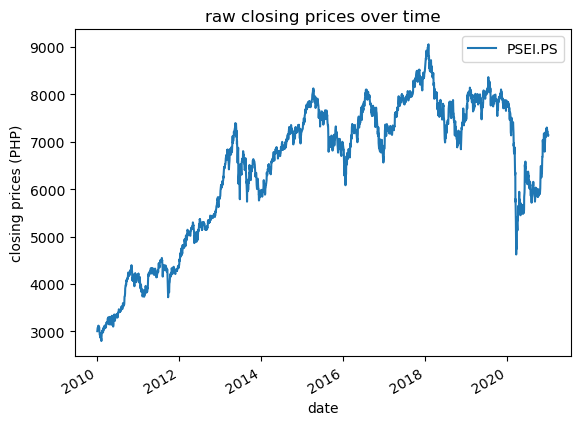
\includegraphics[width=\linewidth]{figure5}
	\end{figure}
	
	The sample period runs from January 1, 2010 to December 31, 2020. After the removal of non trading days we are left with a time series data that has 2671 n successive closing prices of the PSEI. the log returns are computed from the closing prices of each indices.
	
	\begin{figure}[htbp]
		\centering
		\caption{log returns of PSEI}
		\label{fig:log returns}
		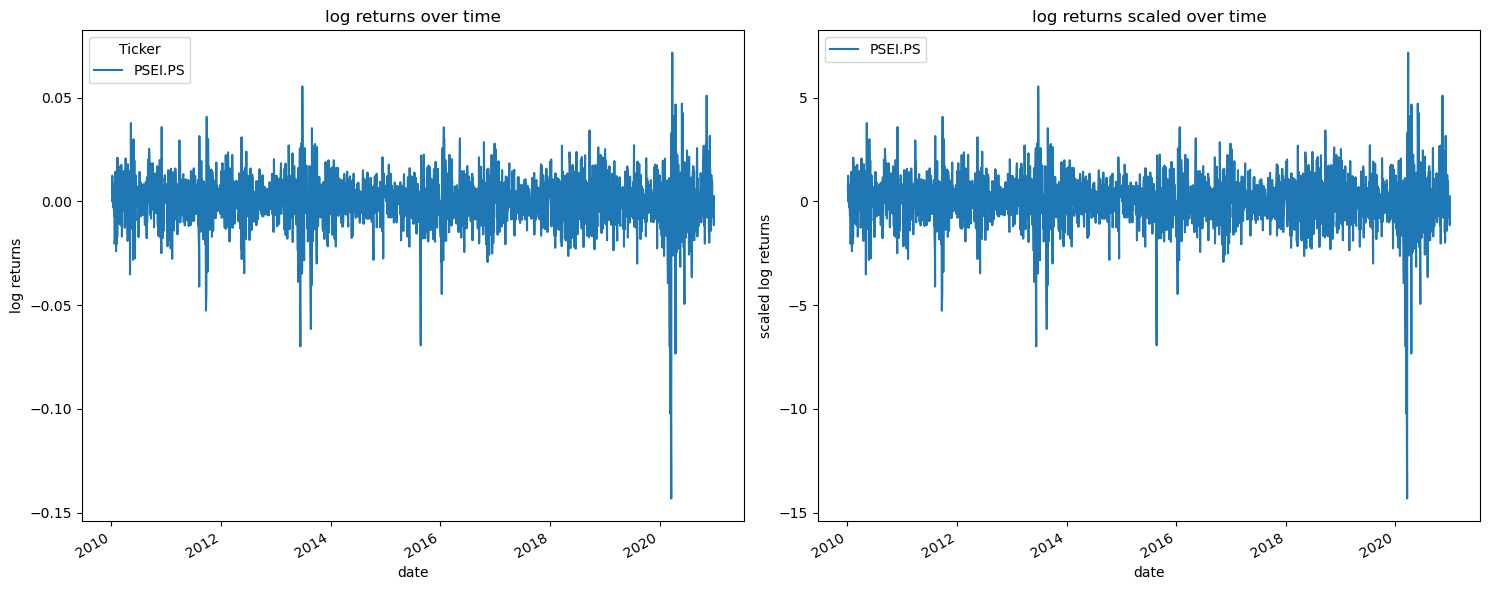
\includegraphics[width=\linewidth]{figure6}
	\end{figure}
	
	
	\begin{table}[htbp]
		\centering
		\caption{Descriptive Statistics of Stock Market Indices}
		\label{tab:desriptive_stats}
		\begin{tabular}{lc}
			\hline
			\textbf{Ticker} & \textbf{PSEI.PS} \\
			\hline
			Mean      & 0.027602  \\
			Std. Dev. & 1.000901  \\
			Skewness  & -0.5155 \\
			Kurtosis  & 2.9254 \\
			\hline
		\end{tabular}
	\end{table}
	
	
	The descriptive statistics confirm the standard stylized facts.
	the series exhibit excess kurtosis exceeding 3, and the PSEI
	displays negative skewness of $-0.5155$, consistent with
	the Skewed-$t$ innovation assumption.
	
	\begin{figure}[htbp]
		\centering
		\caption{density of returns and density of residuals2}
		\label{fig:garch_distributions}
		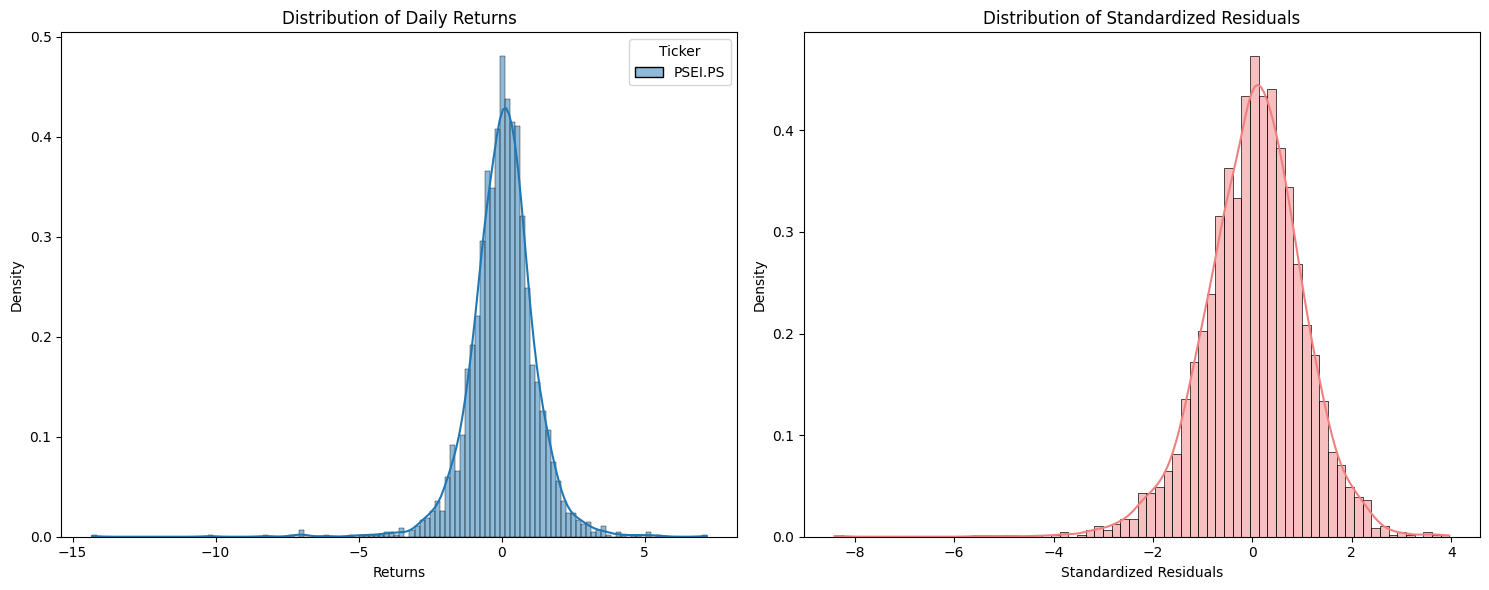
\includegraphics[width=\linewidth]{figure4}
	\end{figure}
	
	The visual confirmations of daily returns did show that the daily returns
	had a fat tailed distribution of excess kurtosis and volatility clustering. With the standardized residuals appear closer to a normal distribution and exhibited absorption of time-varying volatility.
	
	\begin{figure}[htbp]
		\centering
		\caption{Standardized Residuals Over Time}
		\label{fig:garch_standardized_residuals}
		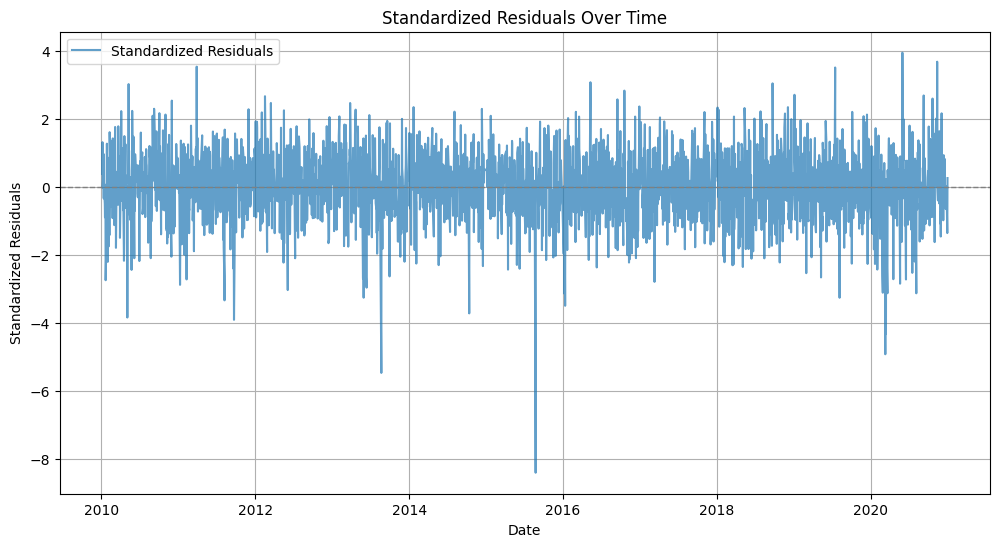
\includegraphics[width=\linewidth]{figure3}
	\end{figure}
	
	The GARCH(1,1) did catch most of the volatility dynamics of the prices generally well within the $2\leq x \leq -2$ it also has no trends or noticeable
	drift showing lack of bias though the model was deeply tested with extreme
	outliers in 2016, heightened residuals on 2010-2012 post great financial crisis hangovers and a spike of 2020 COVID-19 pandemic showing the model is having a hard time capturing the volatility of the closing prices during moments of intense market stress.
	
	The model is implemented in Python.
	Univariate GARCH(1,1) models are estimated via maximum likelihood
	using the \texttt{arch} library and VaR is computed from equation~\eqref{eq:var}.
	
	\begin{table}[htbp]
		\centering
		\caption{Parameter Estimates}
		\begin{tabular}{lcc}
			\hline
			Parameter & Estimate & Std. Error \\
			\hline
			$\hat{\omega}$ & 0.0613 & 0.01522 \\
			$\hat{\alpha}$ & 0.1267 & 0.01985 \\
			$\hat{\beta}$  & 0.8268 & 0.02589 \\
			$\hat{\alpha} + \hat{\beta}$ & 0.9535 & --- \\
			$\hat{\nu}$ & 7.9191 & 1.2310 \\
			$\hat{\lambda}$ & -0.1111 & 0.02605 \\
			\hline
		\end{tabular}
	\end{table}
	
	The estimated persistence parameters $\hat\alpha + \hat\beta$ are 0.9535,
	consistent with the slow volatility decay typical of daily equity data.
	indicating that a shock to Philippine market volatility takes
	approximately $1/(1 - \hat\alpha - \hat\beta) \approx 21.505376344$ as the time constant for mean reversion with a half life formula evaluation of: $\approx 21.505376344 * \ln{2} \approx 14.9$ 	
	days to halve in impact.The estimated degrees-of-freedom parameter $\hat\nu = 7.9191$ confirms significant tail thickness relative to the normal distribution.
	
	Figure~\ref{fig:var} plots the estimated daily 5\% VaR series against
	the realized PSEI losses over the sample period.
	
	\begin{figure}[htbp]
		\centering
		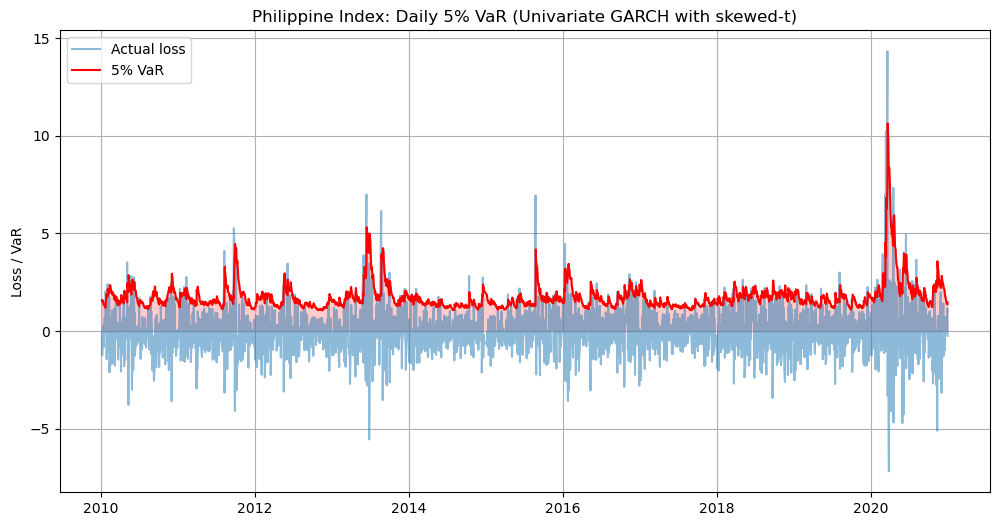
\includegraphics[width=\textwidth]{Figure_1.png}
		\caption{Daily 5\% VaR for the PSEI estimated via GARCH(1,1) (red line)
			versus realized daily losses (blue bars), January 2010 --
			December 2020. A loss observation above the red line constitutes
			a VaR violation.}
		\label{fig:var}
	\end{figure}
	
	Several features are immediately visible.
	During the tranquil mid-cycle period of 2014--2017, the VaR estimate
	stabilizes near $\approx 2.3\%$, reflecting the relatively
	low realized volatility of that era. The estimate rises sharply in response to known stress events: the 2011 Euro-area sovereign debt concerns, the 2013 taper tantrum, and the 2015--2016 China growth scare each produce visible spikes in the VaR line, with the model reacting within one to a few trading days.This responsiveness is a direct consequence of the GARCH
	$\alpha\,\varepsilon_{t-1}^2$ term feeding yesterday's squared shock
	into today's variance estimate.
	
	The dominant feature of the chart is the March 2020 COVID-19 crash.
	The PSEI recorded its largest single-day loss in the sample on
	early 2020, falling $\approx 14\%$
	movement far in excess of any previous observation.
	The GARCH VaR peaked at approximately $10\%$
	during this period, representing the model's real-time recognition
	that the distribution of losses had shifted to a fundamentally
	different regime.
	
	The Kupiec unconditional coverage test assesses whether the
	observed VaR violation rate is statistically consistent with the
	nominal 5\% target.
	Under the null hypothesis that the true violation probability is
	$\alpha = 0.05$, the likelihood ratio statistic
	\begin{equation}
		\text{LR}_{\text{uc}} = 2\left[
		\ln\!\left(\hat p^{n_v}(1-\hat p)^{T-n_v}\right) -
		\ln\!\left(\alpha^{n_v}(1-\alpha)^{T-n_v}\right)
		\right]
		\label{eq:kupiec}
	\end{equation}
	is asymptotically $\chi^2(1)$, where $n_v$ is the number of violations
	and $\hat p = n_v/T$ is the empirical violation rate \parencite{MathWorksVaRBacktesting}.
	
	\begin{figure}
		\centering
		\caption{var with violations crossed}
		\label{fig:var_violation_cross}
		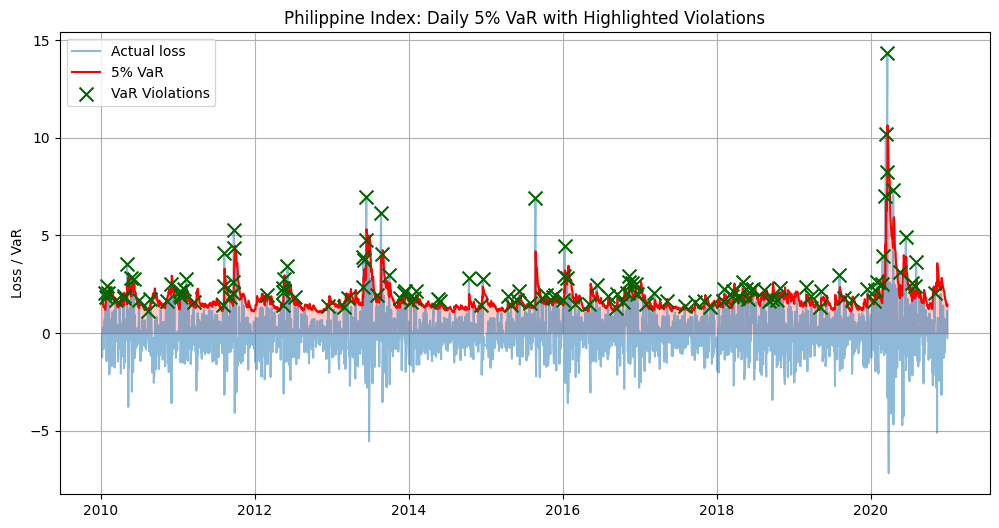
\includegraphics[width=\linewidth]{figure2}
	\end{figure}
	
	\begin{table}[htbp]
		\centering
		\caption{Backtesting Results}
		\begin{tabular}{lc}
			\hline
			Metric & Value \\
			\hline
			Total observations & 2671 \\
			Number of violations & 134 \\
			Violation rate & 0.0502 \\
			Expected violation rate & 0.0500 \\
			Kupiec test (LR statistic) & 0.0016 \\
			Kupiec test ($p$-value) & 0.9681 \\
			\hline
		\end{tabular}
	\end{table}
	
	The estimated violation rate is $\hat p = 0.0502$
	(134 violations out of $T = 2671$ observations),
	and the Kupiec statistic is $\text{LR}_{\text{uc}} = 0.0016$
	with $p$-value $= 0.9681$. The model is statistically
	indistinguishable to the $0.05$ target with $0.0502$ but a p value of $0.9681$ fails to reject the null hypothesis meaning the GARCH(1,1) model has no statistical evidence misspecified for PSEI in terms of violation frequency and that the model adequately captures the downside risks  of the PSEI over the sampled period.

	\section*{Discussion}
		The violation rate shows a higher value which equals 0.0502 than the expected value which equals 0.05 for the 5\% VaR model. The results show that 5.02\% of the data points went beyond the VaR limit which matches the expected results. The model demonstrates excellent risk estimation capabilities because it shows only a minor difference from actual outcomes. The VaR model provides accurate loss assessments because it maintains proper calibration to assess financial risk in the dataset according to its actual performance.
		
		The Kupiec test results show a likelihood ratio of 0.0016 and a p-value of 0.9681. The null hypothesis must remain intact because the p-value exceeds 0.05. The actual violation rate matches the expected 5\% level based on statistical testing. The VaR model does not have any statistical evidence that shows it is incorrect. The model succeeds in passing the Kupiec test because it delivers accurate and trustworthy risk predictions.
		
		The graph shows actual loss data compared to the 5\% VaR line which demonstrates that most actual loss values stay below the VaR line except for few cases when losses surpass it. The 5\% VaR model shows expected violations through its exceedances which demonstrate actual loss values. The actual loss and VaR show noticeable spikes which start in later periods including the time period close to 2020 because markets become more volatile. The model demonstrates risk level changes through its upward adjustment of the VaR line during these periods. The GARCH model successfully captures fluctuations in volatility which occur over different time periods.
		
		While the model successfully controlled the majority of data points, it struggled with infrequent and extreme market disruptions, such as the negative drop in 2016 that reached beyond -8. In these instances, the model required multiple steps to re-establish baseline levels, indicating a potential lag during sudden exceptional events.The current study is limited in scope as the data focuses exclusively on the PSEI.PS ticker from 2010 to 2020, meaning market behaviors prior to 2010 were not analyzed and the findings may not be applicable to other types of global markets. Since the GARCH model was constructed based on the specific volatility patterns of the Philippine Index within this decade. Statistical properties  might differ significantly in developed markets or other emerging markets. Furthermore, while the model is proficient at handling standard market turbulence, it faces challenges in predicting high market stress events that fall outside the historical trends of the selected time frame.
		
		Overall the study has showed that GARCH is applicable to PSEI in determining the Value at Risk modeling with some modification due to the skewness of the data the Back-test for the Value at Risk exhibited that analytically the model has captured most of the regular market environment of the PSEI closing prices volatility with exceptions to extremely outlier events such as Covid-19 and other statistical outliers here and there. The study is a expository of the PSEI under the 2010s  to 2020 and that findings here do not universally apply to other markets. It is highly recommended for readers to reproduce the methodology before assuming findings here applies everywhere.
		

	\printbibliography[heading=bibintoc]
	
	\section*{Appendix}
	
		\begin{table}[htbp]
			\centering
			\begin{tabular}{lclc}
				\toprule
				\textbf{Dep. Variable:} &            PSEI.PS            & \textbf{  R-squared:         } &     0.000   \\
				\textbf{Mean Model:}    &           Zero Mean           & \textbf{  Adj. R-squared:    } &     0.000   \\
				\textbf{Vol Model:}     &             GARCH             & \textbf{  Log-Likelihood:    } &   -3822.40  \\
				\textbf{Distribution:}  & Standardized Skew Student's t & \textbf{  AIC:               } &    7654.79  \\
				\textbf{Method:}        &       Maximum Likelihood      & \textbf{  BIC:               } &    7684.24  \\
				\textbf{}               &                               & \textbf{  No. Observations:  } &    2672     \\
				\textbf{Date:}          &        Sun, Apr 12 2026       & \textbf{  Df Residuals:      } &    2672     \\
				\textbf{Time:}          &            13:54:57           & \textbf{  Df Model:          } &     0       \\
				\bottomrule
			\end{tabular}
			\begin{tabular}{lccccc}
				& \textbf{coef} & \textbf{std err} & \textbf{t} & \textbf{P$> |$t$|$} & \textbf{95.0\% Conf. Int.}  \\
				\midrule
				\textbf{omega}    &       0.0613  &    1.522e-02     &     4.027  &      5.639e-05       &   [3.147e-02,9.115e-02]     \\
				\textbf{alpha[1]} &       0.1267  &    1.985e-02     &     6.381  &      1.759e-10       &    [8.775e-02,  0.166]      \\
				\textbf{beta[1]}  &       0.8268  &    2.589e-02     &    31.930  &      1.019e-223      &     [  0.776,  0.878]       \\
				& \textbf{coef} & \textbf{std err} & \textbf{t} & \textbf{P$> |$t$|$} & \textbf{95.0\% Conf. Int.}  \\
				\midrule
				\textbf{eta}    &       7.9191  &        1.231     &     6.431  &      1.271e-10       &     [  5.505, 10.333]       \\
				\textbf{lambda} &      -0.1111  &    2.605e-02     &    -4.265  &      1.997e-05       &    [ -0.162,-6.006e-02]     \\
				\bottomrule
			\end{tabular}
			%\caption{Zero Mean - GARCH Model Results}
		\end{table}
		
		\begin{table}[htbp]
			\centering
			\caption{Descriptive Statistics for Returns}

		\begin{tabular}{lr}
			\toprule
			Ticker & PSEI.PS \\
			\midrule
			count & 2671.000000 \\
			mean & 0.032118 \\
			std & 1.188711 \\
			min & -14.322357 \\
			25\% & -0.569004 \\
			50\% & 0.057292 \\
			75\% & 0.657294 \\
			max & 7.171699 \\
			\bottomrule
		\end{tabular}
				\end{table}
				
		\begin{table}
			\caption{Descriptive Statistics for Actual Loss (Loss = -Return)}
			\centering	
		\begin{tabular}{lr}
			\toprule
			Ticker & PSEI.PS \\
			\midrule
			count & 2671.000000 \\
			mean & -0.032118 \\
			std & 1.188711 \\
			min & -7.171699 \\
			25\% & -0.657294 \\
			50\% & -0.057292 \\
			75\% & 0.569004 \\
			max & 14.322357 \\
			\bottomrule
		\end{tabular}
				\end{table}
		
		\begin{table}
			\centering
						\caption{Descriptive Statistics for 5\% VaR Forecasts}
		\begin{tabular}{lr}
			\toprule
			& conditional vol \\
			\midrule
			count & 2671.000000 \\
			mean & 1.757217 \\
			std & 0.723723 \\
			min & 1.063220 \\
			25\% & 1.370080 \\
			50\% & 1.592244 \\
			75\% & 1.897558 \\
			max & 10.633742 \\
			\bottomrule
		\end{tabular}
				\end{table}
		\begin{table}
			\centering
						\caption{Descriptive Statistics for Standardized Residuals}
		\begin{tabular}{lr}

			\toprule
			& 0 \\
			\midrule
			count & 2672.000000 \\
			mean & 0.027602 \\
			std & 1.000901 \\
			min & -8.404813 \\
			25\% & -0.565267 \\
			50\% & 0.062232 \\
			75\% & 0.656553 \\
			max & 3.959610 \\
			\bottomrule
		\end{tabular}
				\end{table}
		
		
	
\end{document}